\documentclass[a4paper,12pt]{article}
\usepackage{sbc-template}
\usepackage{graphicx,url}
%\usepackage[brazil]{babel}
%\usepackage[none]{hyphenat} 
%\usepackage[latin1]{inputenc}  
\usepackage[utf8]{inputenc} 
\usepackage{hyperref}
\usepackage{natbib}
% UTF-8 encoding is recommended by ShareLaTex
     
%\sloppy

\title{Análise Estatística da Expressão do Gene CD274 em Tecidos com Câncer\\
Statistical Analysis of CD274 Gene Expression in Tissues with Cancer}

\author{Odilon J. dos Santos\inst{1}}

\address{Instituto Metrópole Digital\\
 Universidade Federal do Rio Grande do Norte
  (UFRN)\\
  Natal -- RN -- Brasil\\
  Disciplina: PROJETOS EM BIOINFORMÁTICA\\
  Orientadora: Profa. Dra. Tirzah Braz Petta Lajus\\
  \email{odilonjulio@ufrn.edu.br}
}

\begin{document} 

\maketitle

\begin{abstract}
  This is the analysis of the possible correlation between gene expression
  of the PD-L1 (CD274) gene in cancer tissues, more specifically, in this case,
  cancer of the skin and lungs of about 500 individuals and their respective
  after diagnosis.
\end{abstract}
     
\begin{resumo} 
 Trata-se da análise da possível correlação existente entre a expressão gênica
 do gene PD-L1 (CD274) em tecidos com câncer, mais especificamente, neste caso,
 câncer de pele e de pulmão, de cerca de 500 indivíduos e a suas respectivas 
 sobrevidas, após diagnosticados. 
\end{resumo}


\section{Introdução} \label{sec:firstpage}

\begin{figure}[h!]
\centering

\includegraphics[width=1 \textwidth]{pdl1.jpg}
\caption{Proteína PD-L1}
\label{fig:PD-L1}
\end{figure}

O ligante de morte programada 1 (PD-L1), também denominado como B7-H1, é uma
proteína que, em humanos, é codificada pelo gene CD274. Estudos especulam que 
ele exerce papel fundamental na supressão do sistema imunológico, causando a redução
da proliferação das células T, que são os glóbulos brancos responsáveis pela defesa
do organismo diante de antígenos.

Dentre as possibilidades de tratamento de alguns tipos de câncer, segue emergente
a terapia baseada na tentativa de regular a expressão gênica do PD-L1. Desta forma, 
a análise apresentada a seguir é um estudo introdutório que visa descobrir, estatisticamente,
 se há relação entre a sobrevida de indivíduos com dois tipos de câncer específicos 
 (pulmão e pele) e a expressão do gene CD274 nos referidos tecidos.

\section{Objetivos} \label{sec:firstpage}

Diante da justificativa acima, o objetivo central dessa análise inicial é quantificar o quão importante é, para o tratamento de alguns tipos de câncer, o controle ou regulação da expressão gênica do gene CD274
por meio de inibidores (anti-PDL1).

Especificamente, e paralelamente, foram analisados os dois tecidos
com câncer, acima referidos. Mas pesquisas futuras estão direcionadas aos demais tecidos e, além disso,
às demais doenças ou eventos específicos do organismo.

\section{Metologia} \label{sec:firstpage}

\begin{figure}[h!]
\centering
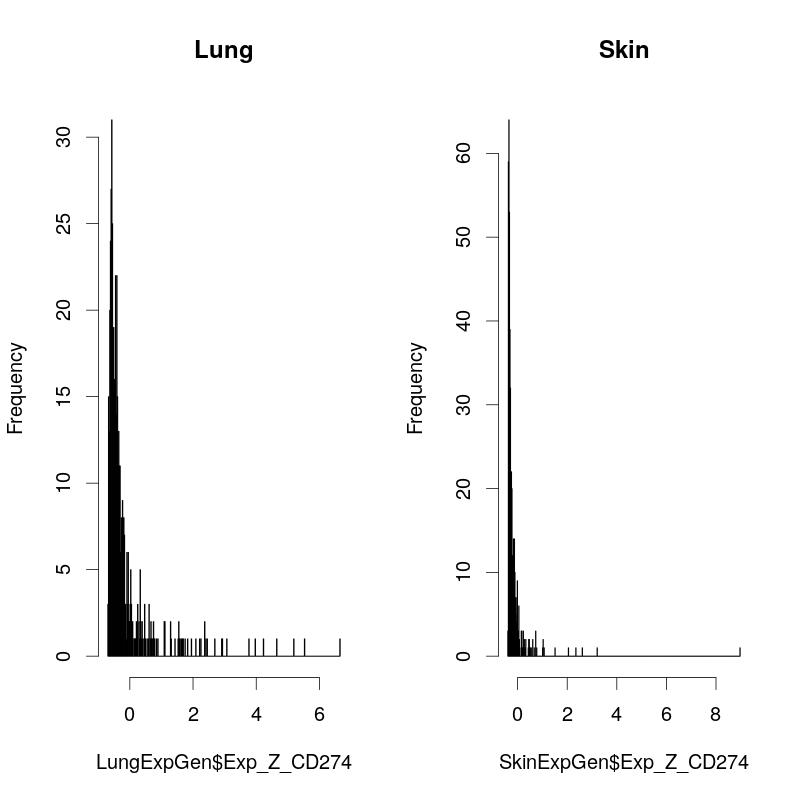
\includegraphics[width=0.7 \textwidth]{plot_histogramas.jpeg}
\caption{Histogramas da Expressão Gênica do CD274}
\label{fig:Hist1}
\end{figure}

Inicialmente, foram coletados dados do portal \href{https://www.cbioportal.org/}{cBioPortal}, os quais
relacionam pacientes que possuem, paralelamente, câncer de pulmão e de pele. Em ambos os casos, foi
quantificada em RPKM (Reads Per Kilobase Million) a expressão do gene CD274, avaliada em algum momento do tratamento, e o tempo de vida do respectivo paciente, após diagnóstico, até o período da alimentação do banco 
de dados ou, em caso de morte, do seu falecimento.



\begin{figure}[h!]
\centering
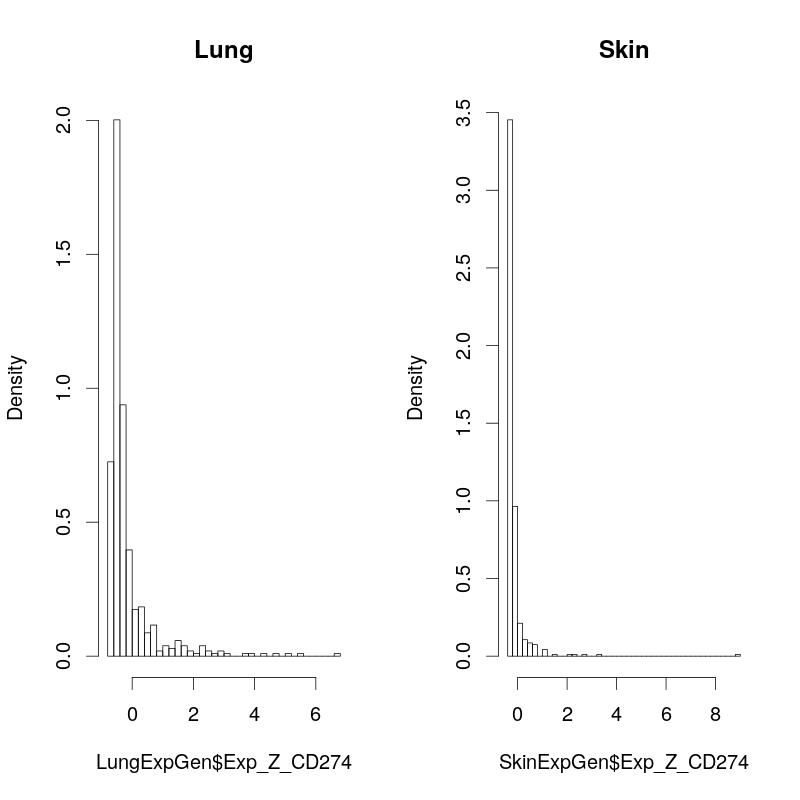
\includegraphics[width=0.7 \textwidth]{plot_histograma2.jpeg}
\caption{Histogramas da Expressão Gênica do CD274 normalizado.}
\label{fig:Hist2}
\end{figure}

Com intuito de permitir melhor avaliação e estudo dos dados, foi utilizado o \href{https://www.r-project.org/}{Software R} e suas principais bibliotecas com fim criar um \textit{script} padronizado que, futuramente, pode ser utilizado para avaliar outros pacientes.


Com auxílio do R, os valores da expressão gênica dos indivíduos foram normalizados em \textbf{Z-Score} e ordenados. Em seguida, tal distribuição foi avaliada graficamente e, por meio do \textbf{Teste de Shapiro-Wilk}, constatou-se não se tratar de uma distribuição normal. Tal fato já aponta para a suspeita que a expressão gênica do CD 274 não segue um padrão "bem definido", pelo menos nesses pacientes, e que seus extremos não estão equidistantes do média expressão gênica.

\begin{figure}[h!]
\centering
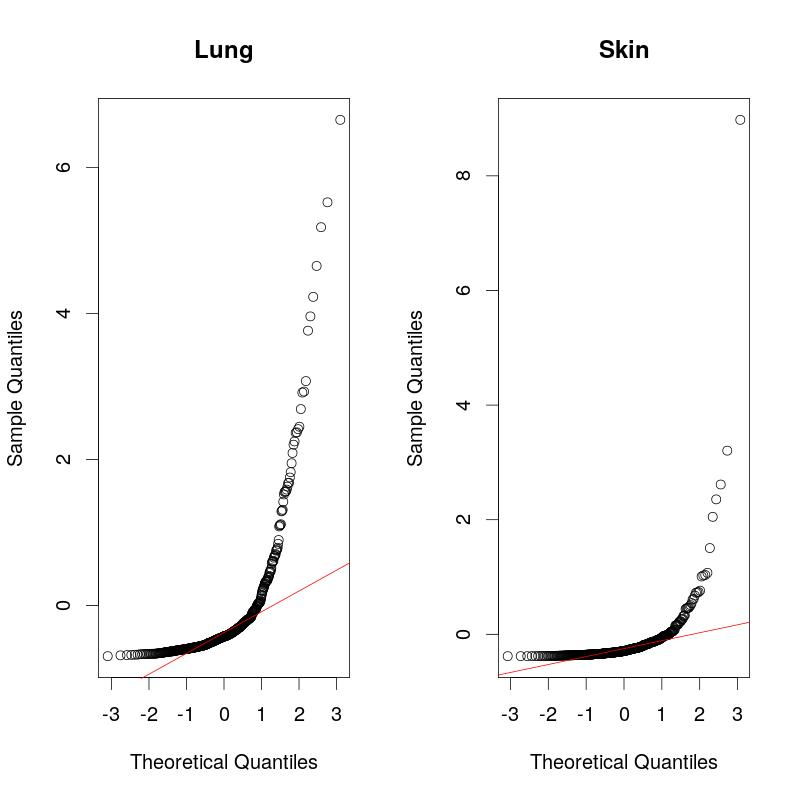
\includegraphics[width=0.5 \textwidth]{plot_testeNorm.jpeg}
\caption{Teste que constata que a distribuição da expressão gênica não segue uma distribuição normal.}
\label{fig:TesteNorm}
\end{figure}

Continuando a análise, foram captados os indivíduos que representam os 5\% com maior expressão gênica e os 5\% com menor expressão. Tais indivíduos tiveram uma análise secundária, onde foi correlacionada a sobrevida de cada um, em meses, deles e seus respectivos valores (em Z-Score) de expressão do gene em tela. Após tal refino, foi possível conjecturar que há, de fato, em números, uma relação direta entre o gene CD274 estar superexpresso e a baixa sobrevida dos pacientes.

\begin{figure}[h!]
\centering
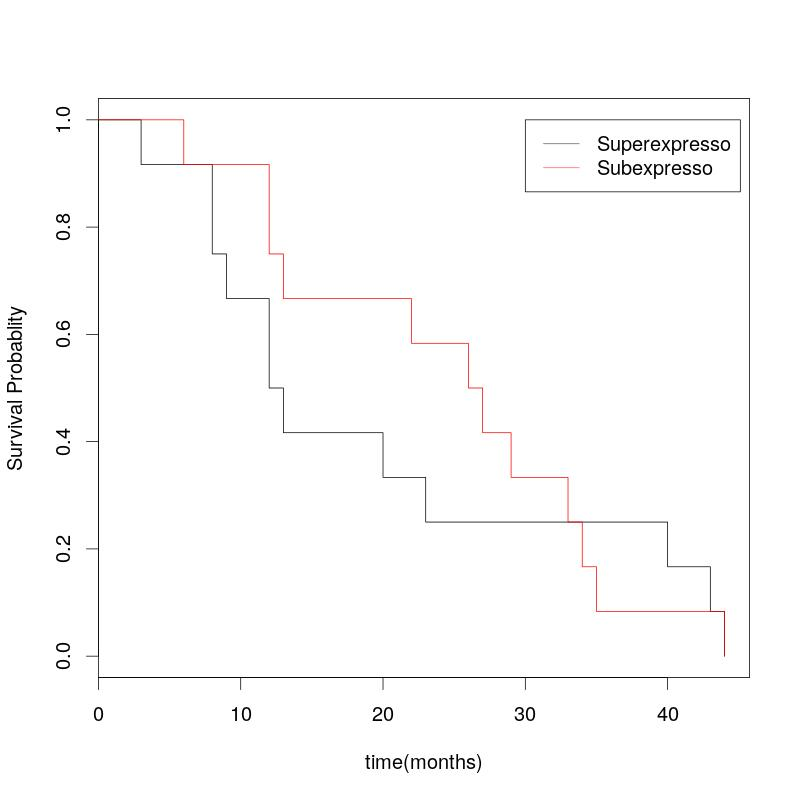
\includegraphics[width=0.5\textwidth]{plot_AnaliseSobrevida.jpeg}
\caption{Curva de Kaplan-Meier da Análise de Sobrevida.}
\label{fig:TesteNorm}
\end{figure}

É importante lembrar que esse estudo foi realizado com uma banco de dados muito pequeno e se faz necessário um maior aprofundamento nas análises. Contudo, ainda será realizado um teste de hipótese estatística para reafirmar ou confrontar a informação encontrada até então.

Desta forma, essa investigação, pelo pequeno número de amostras até então avaliadas, ainda é inconclusiva, mas ascende a expectativa real de que a relação aqui encontrada tem grande probabilidade de também existir numa população com maior número de indivíduos. 

Por fim, vale salientar que foram avaliados pacientes que ainda possuíam o câncer e/ou faleceram em decorrência da doença, já que apenas ficou perceptível que o gene pode estar superexpresso em indivíduos livres da doença.

Há, então, uma proposta de criação de script padronizado ou software que faça tais análises estatísticas, tratando o dado e verificando a expressão de genes sua relação com a sobrevida do paciente com câncer, apresentando, por fim, a curva de subrevida do Kaplan-Meier. 

Mais informações que justificam essa análise podem ser encontradas em \cite{brahmer2012safety}, \cite{reck2016pembrolizumab}, \cite{iwai2002involvement} e outros que facilmente podem ser encontrados em conteúdo público.

\bibliographystyle{sbc}
\bibliography{ref}

\end{document}
